\documentclass[11pt,answers]{exam}
\usepackage[utf8]{inputenc}
\usepackage[french]{babel}
\usepackage[T1]{fontenc}
\frenchbsetup{StandardLists=true}
\usepackage{amssymb,amsmath,amsfonts}
\usepackage{lmodern}
\usepackage{enumitem}
\usepackage{url}
\usepackage{hyperref}
\usepackage{graphicx}
\usepackage{listings}
\usepackage{xcolor}
\usepackage{tikz}
\usetikzlibrary{calc, shapes, backgrounds}
\usepackage{pgfpages}
\DeclareMathAlphabet{\mathcal}{OMS}{cmsy}{m}{n}
\usepackage{pgf}
\usetikzlibrary{arrows,automata,calc,positioning}
\usepackage{listings}

\definecolor{codegreen}{rgb}{0,0.6,0}
\definecolor{codegray}{rgb}{0.5,0.5,0.5}
\definecolor{codepurple}{rgb}{0.58,0,0.82}
\definecolor{backcolour}{rgb}{0.95,0.95,0.92}
\definecolor{myOrange}{rgb}{0.85,0.325,0.098}
\definecolor{myMidBlue}{rgb}{0,0.4,0.663}
\newcommand{\edit}[1]{\textcolor{myMidBlue}{#1}}
\newcommand{\error}[1]{\textcolor{red}{\bf #1}}

\lstdefinestyle{mystyle}{
    backgroundcolor=\color{backcolour},   
    commentstyle=\color{codegreen},
    keywordstyle=\color{magenta},
    numberstyle=\tiny\color{codegray},
    stringstyle=\color{codepurple},
    basicstyle=\ttfamily\footnotesize,
    breakatwhitespace=false,         
    breaklines=true,                 
    captionpos=b,                    
    keepspaces=true,                 
    numbers=left,                    
    numbersep=5pt,                  
    showspaces=false,                
    showstringspaces=false,
    showtabs=false,                  
    tabsize=2
}
\lstset{style=mystyle}

\footer{}{Page~\thepage}{}

\begin{document}
\noindent
LEPL1108 - Mathématiques discrètes et probabilité \hfill Année académique 2023--2024\\[-2mm]
\rule{\linewidth}{0.5pt}

\begin{center}

{\large Devoir 3 : Puissance 4 (\textit{Monte Carlo})}
\bigskip

\end{center}
\hrule
\bigskip

\section*{Informations pratiques}
\noindent

\noindent
\emph{Ce devoir est individuel.} Nous vous encourageons à échanger vos idées entre vous sur la façon d'aborder ce devoir. En revanche, votre solution doit être rédigée individuellement: ne partagez pas votre production ! Nous serons intransigeants si nous observons des similitudes dans votre code ou votre rapport, lesquels passeront dans les logiciels anti-plagiat de Gradescope.

\bigskip \noindent
\emph{Echéance:} Mercredi 29 Décembre 2023 à 18h00.

\bigskip


\noindent
\section*{Soumission}
\begin{itemize}
\setlength{\itemsep}{0mm}
	\item Soumission sur \url{https://www.gradescope.com/}, connectez-vous avec vos identifiants UCLouvain.
	\item Vous devriez voir apparaître LEPL1108 dans la liste de vos cours. Si ce n'est pas le cas, vous devriez pouvoir rejoindre le cours en vous servant du code \texttt{6GGV63}.
    \item Ce devoir est divisé en quatre sections. Les sections 1, 2 et 4 doivent être complétées en répondant aux questions par écrit et en soumettant l'énoncé complété en PDF sur Gradescope dans la partie \texttt{Devoir 3: Puissance 4 PDF}. Le code de la section 3 doit être soumis sur Gradescope dans la partie \texttt{Devoir 3: Puissance 4 AI}.
    \item Un fichier Latex intitulé \texttt{Devoir3.tex} est disponible sur Moodle pour faciliter le remplissage de l'énoncé du devoir. Ne modifier pas la taille et/ou la position des cadres de réponse pour éviter des problèmes de lecture par Gradescope.
	\item Pour les codes, respectez le modèle fourni, vous risquez sinon d’avoir des problèmes de codage ou des problèmes de lecture du code par Gradescope.
    \item Sur Moodle, vous trouverez un fichier "squelette" \texttt{montecarlo.py} à compléter et un fichier \texttt{connect4.py} qui seront fournis pour les sections 2 et 4 ainsi qu'un fichier "squelette" \texttt{ai\_student.py} à compléter pour la section 3.
	\item Pour la section 3, les seuls packages autorisés sont: \texttt{numpy}, \texttt{math} et \texttt{random}.
    \item Pour ce devoir, l'appellation joueur 1/player 1 désigne le joueur ou la joueuse qui entame la partie.
    \item \textbf{Pondération des points: Les sections 3 et 4 du devoir sont des questions de dépassement et compteront comme bonus pour ce devoir. Un bonus supplémentaire sera également attribué aux étudiants et étudiantes qui obtiendront les meilleurs scores pour les sections 3 et 4.}
\end{itemize}


\newpage

\section*{Introduction}

Nous vous proposons de jouer un jeu que vous connaissez toutes et tous : le Puissance 4. Pour celles et ceux qui ne sont pas familiers avec ce jeu, les règles peuvent être trouvées sur le site suivant: \href{https://www.regles.com/jeux/puissance-4.html}{https://www.regles.com/jeux/puissance-4.html}. Etant toutes et tous des grands amateurs de calcul probabiliste, nous utiliserons la méthode dite de Monte Carlo pour calculer le pourcentage de victoire attendu à Puissance 4 pour différentes stratégies de jeu. 

\medskip

\section{Borne inférieure} \label{sec:borne_inf}

Afin de calculer exactement des probabilités de succès ou d'échec dans ce jeu, il faudrait explorer toutes les parties possibles. Or, on soupçonne que ce nombre est important. Dans cette section, on calcule une borne inférieure sur le nombre de parties possibles, afin de soutenir notre intuition et justifier le recours à la méthode de Monte Carlo.

On propose un calcul simple de borne inférieure. Peu importe que cette borne soit proche ou non du nombre exact de parties possibles (que vous pouvez trouver en quelques clics sur Google). Notre borne peut être grossière, il suffit qu'elle soit assez grande pour justifier notre recours à Monte Carlo.

On considère l'état du plateau représenté en Figure \ref{fig:bound}, et on demande de dénombrer toutes les parties possibles qui ont pu mener à un tel état du plateau de jeu. Bien que de nombreuses bornes inférieures puissent être proposées, ici on s'attend au nombre exact de parties ayant mené au plateau de la Figure \ref{fig:bound} -- il n'y a qu'une seule bonne réponse. Justifiez votre réponse en expliquant votre raisonnement.

\textbf{NB:} Afin que les choses soient claires, deux parties sont considérées comme différentes si les coups ne sont pas joués dans le même ordre.

\begin{figure}[!ht]
	\centering
	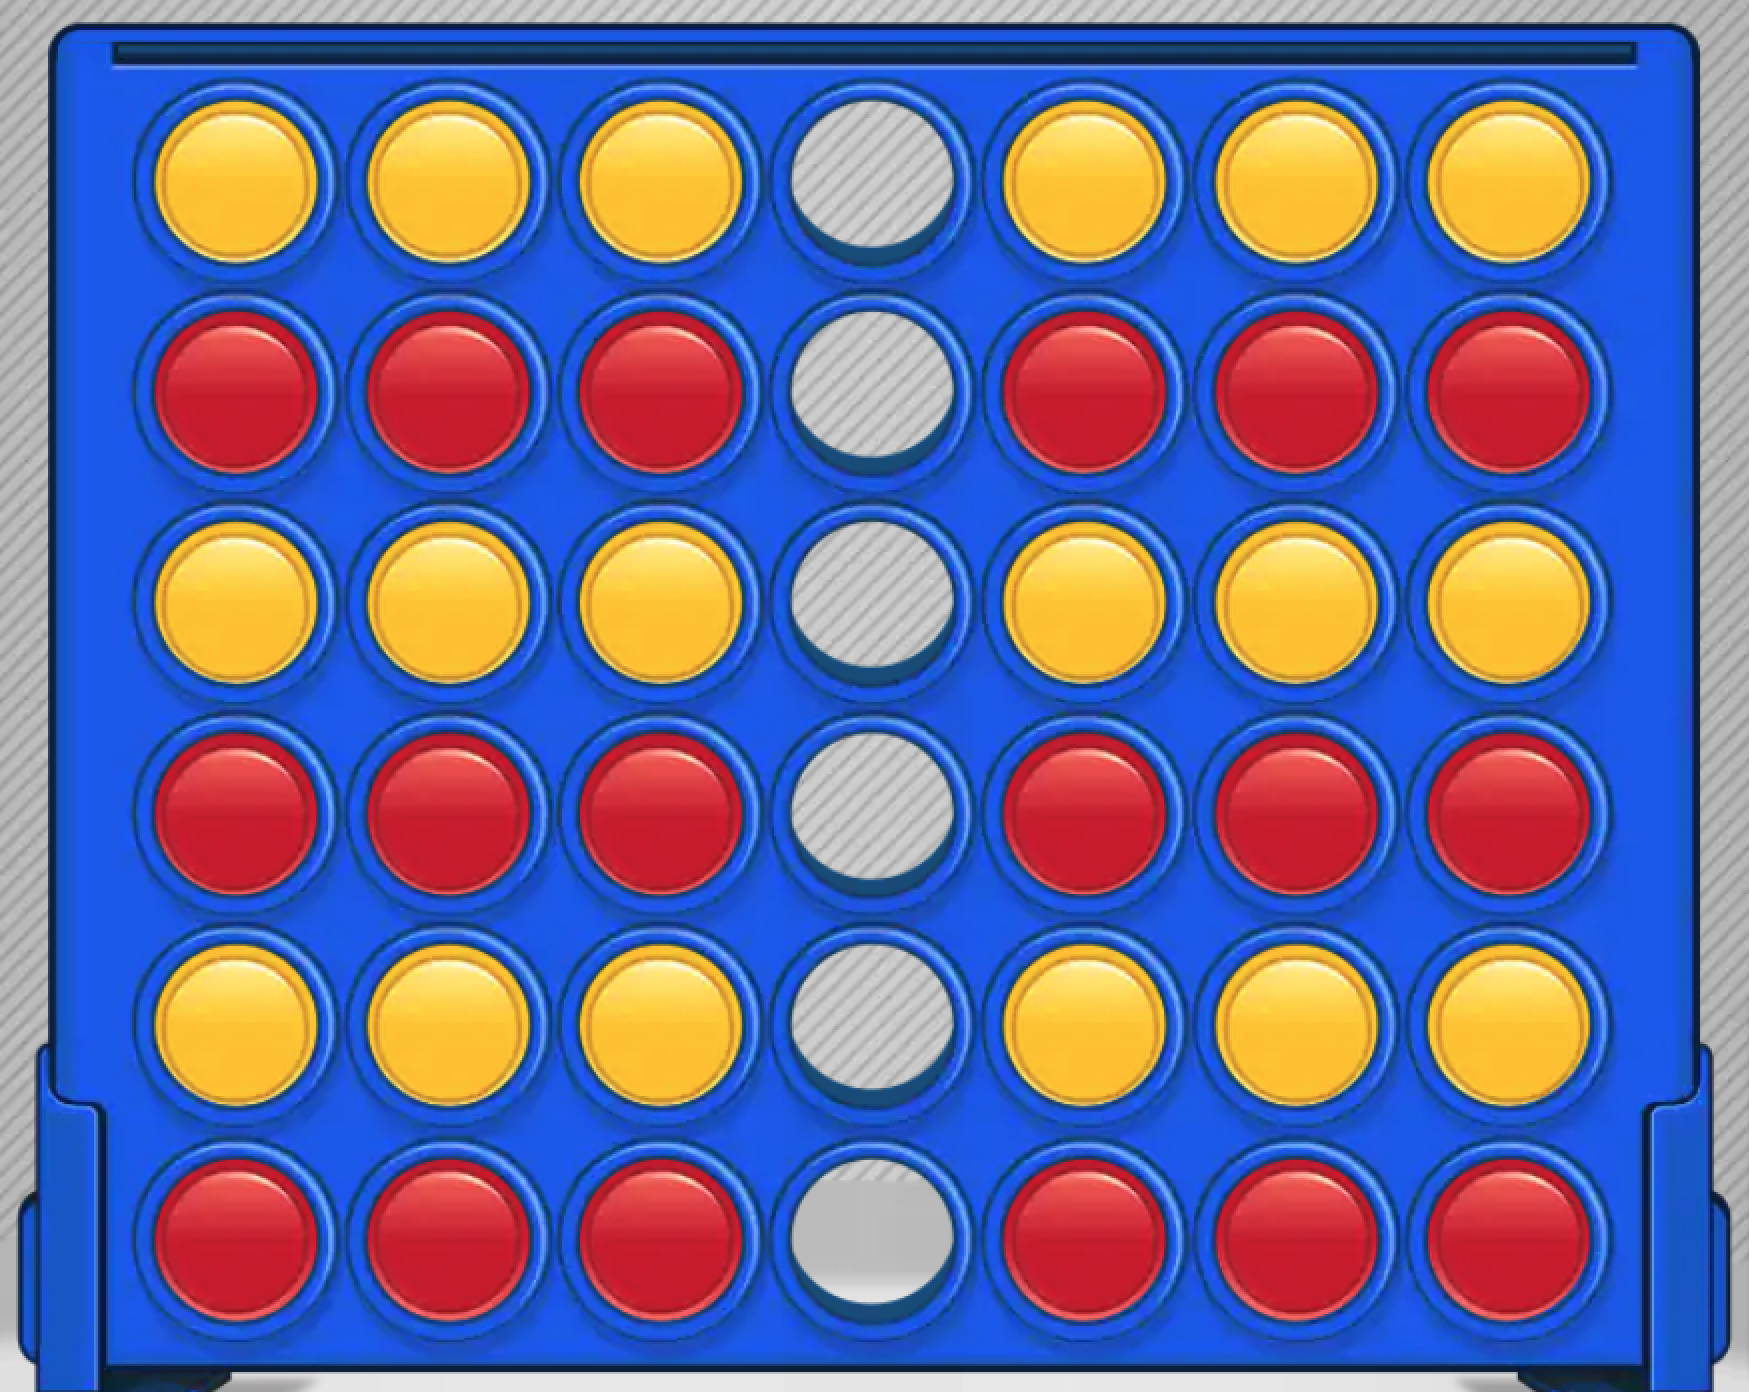
\includegraphics[width=0.6\textwidth]{board.png}
 	\caption{Plateau de jeu considéré pour le calcul de borne inférieure}
	\label{fig:bound}
\end{figure}

\begin{solutionbox}{210mm}
Le joueur jaune n'a aucune influence sur le jeu en raison de la disposition du plateau, il est obligé de suivre le joueur rouge. Nous nous intéressons donc uniquement au joueur rouge. On constate que le joueur rouge joue 18 coups au cours de sa partie. Il y a donc 18 permutations possibles pour les coups joués par le joueur rouge. Cependant, on constate que certaines permutations défient la gravité.

En effet, on ne peut pas permuter l'ordre de coups situés l'un au-dessus de l'autre. Il y a donc 3 coups par colonne, et donc 3! permutations à supprimer par colonne.

Pour éliminer les permutations impossibles, il nous suffit de diviser le nombre total de permutations par le nombre de permutations indésirables.
On obtient donc $\frac{18!}{(3!)^6} = 1.2 \times 10^{11}$
 parties possibles. Le exposant 6 est dû au fait qu'il y a 6 colonnes.

\end{solutionbox}

\newpage

\section{Méthode de Monte Carlo}

Dans cette section, nous considérons une stratégie de jeu très basique : \texttt{ai\_random}. Cette stratégie fonctionne de la manière suivante :
\begin{itemize}
    \item S'il y a un coup gagnant à jouer (c'est-à-dire une ligne de trois jetons de sa couleur, avec une place libre à côté), il est joué, c'est un \texttt{attack move.}
    \item Sinon, s'il y a un coup gagnant pour l'adversaire, ce coup là est joué, afin de bloquer une potentielle victoire de l'adversaire au prochain tour, c'est un \texttt{defense move.}
    \item Sinon, un coup est fait au hasard parmi les colonnes non-remplies.
\end{itemize}

Nous nous intéressons à la question suivante : si la stratégie \texttt{ai\_random} joue contre elle-même, quel est l'avantage à entamer la partie ? Plus précisément, si les deux joueurs suivent la stratégie \texttt{ai\_random}, quelle est la probabilité que le joueur 1 (celui qui commence) gagne, la probabilité que le joueur 2 gagne, et la probabilité d'ex-æquo ?

La borne inférieure obtenue en section \ref{sec:borne_inf} montre que calculer ces probabilités de manière exacte n'est pas gérable en temps de calcul sur votre ordinateur. C'est pourquoi nous avons recours à la méthode dite de Monte Carlo afin d'approximer ces probabilités.

La méthode de Monte Carlo consiste à estimer ces probabilités en simulant un grand nombre de parties, et en comptant le nombre de victoires et d'ex-æquo pour ces parties simulées. Nous nous intéressons aussi à l'évolution de l'estimé obtenu en fonction du nombre de parties jouées : plus le nombre de parties jouées est élevé, plus l'estimé sera bon.

Il vous est demandé de calculer le pourcentage de victoires du joueur 1 et le pourcentage d'ex-æquo pour 10, 100, 1000 et 10000 parties. A chaque fois, répétez l'expérience dix fois. Représentez sur un graphique le résultat obtenu pour chacune des dix expériences, ainsi que la moyenne de ces dix expériences. Pour ce faire, les fichiers suivants vous sont fournis:

\begin{itemize}
    \item \texttt{connect4.py} : fichier qui réunit toutes les fonctions nécessaires afin de simuler une partie de Puissance 4:
    \begin{itemize}
        \item \texttt{ai\_random}: la stratégie basique considérée dans cette section.
        \item \texttt{update\_board}: met à jour le tableau de jeu à l'aide du coup reçu en argument.
        \item \texttt{print\_board}: permet une visualisation de l'état du jeu. Utile pour les sections 3 et 4 lorsque vous coderez votre propre AI, et pour débugger.
        \item \texttt{check\_win}: vérifie si le dernier coup joué est gagnant.
        \item \texttt{run\_game}: joue une partie de Puissance 4, et retourne 1 si le 1e joueur l'emporte, 2 si c'est le second et 0 si c'est ex-æquo.
    \end{itemize}
    Pour cette section, vous ne devez pas modifier ce fichier, mais seulement utiliser la fonction \texttt{run\_game} afin de simuler des parties.
    \item \texttt{montecarlo.py} : script à compléter qui simule des parties puis représente graphiquement les résultats obtenus. Le format du graphique est fixé, on vous demande de ne pas le modifier afin de faciliter la correction. La partie du code à compléter vise à calculer les tableaux \texttt{win1} et \texttt{draw} : les résultats des simulations.
\end{itemize}

Insérez votre graphique dans le cadre ci-dessous. Il est normal que votre code prenne $\sim$ 15 min à tourner sur votre machine pour $10^4$ parties.

\begin{solutionbox}{100mm}
    Insérez votre graphique ci-dessous, à la place de ce graphique vide.

    \centering
    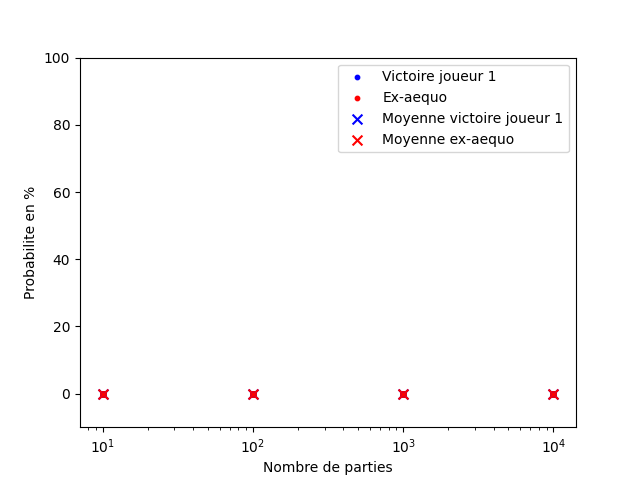
\includegraphics[width=0.75\textwidth]{MCplot_empty.png}
\end{solutionbox}

Sur base du graphique obtenu, répondez aux questions suivantes :

\medskip

1. Y a-t-il un avantage à commencer la partie ? Justifiez votre réponse sur base de votre graphique, en mentionnant les probabilités moyennes obtenues pour $10^4$ parties.
    
\begin{solutionbox}{25mm}
Oui il y a un grand avantage a commencer la partie en 1e comme un peu le voir sur le graphe le joueur qui commence en premier à bien plus de chance de gagner que le joueur 2.

\end{solutionbox}

\medskip

2. Soit $n$ le nombre de parties simulées. Pour un $n$ fixé, on s'intéresse à la distance typique des résultats des dix expériences par rapport à leur moyenne. Sur base de votre graphique, vous observez que cette distance typique évolue (à une constante multiplicative près) en :
\begin{align*}
      (i) \ n^2 \qquad  (ii) \ n \qquad  (iii)\  \sqrt{n} \qquad (iv) \ 1/\sqrt{n} \qquad  (v) \  1/n^2
\end{align*}
Justifiez votre réponse sur base de votre graphique. Cette notion sera approfondie en cours.

\begin{solutionbox}{25mm}
On peut voir que la distance evolue en 1/sqrt(n)

\end{solutionbox}

\newpage

\section{Codez votre propre intelligence artificielle}

Maintenant que nous avons analysé ce qui se passerait avec deux joueurs qui jouent une stratégie aléatoire \texttt{ai\_random}, nous vous proposons d’aller un cran plus loin et de coder votre propre intelligence artificielle (IA) qui joue à Puissance 4. 
Pour tester le bon fonctionnement de votre IA, nous avons préparé une série de tests sur Gradescope de situations critiques pendant une partie de Puissance 4 où votre IA devrait prendre la meilleure décision possible (c.-à-d. choisir de jouer la colonne qui maximise la chance du joueur à gagner). Votre but est de jouer le meilleur coup possible en prenant en compte l'état actuel du plateau de jeu avant votre tour.

\medskip

Il vous est demandé d'implémenter en Python votre IA \texttt{ai\_student.py}, sous la forme d'une fonction dont la signature est donnée ci-dessous :

\lstinputlisting[language=Python]{ai_student.py}


\subsubsection*{Inputs}

\begin{itemize}
	\item \texttt{board} est un tableau (array) numpy de taille $6 \times 7$ qui ne peut contenir que les chiffres 0, 1 ou 2 (0 signifiant que la case est vide, 1 signifiant que la case est remplie par un jeton du joueur 1 et 2 signifiant que la case est remplie par un jetton du joueur 2. Les indexes du tableau font de haut en bas et de gauche à droite, c'est-à-dire que $(0,0)$ correspond au coin en haut à gauche et $(6,7)$ correspond au coin en bas à droite.
	Le tableau représente l'état actuel du plateau de jeu à votre tour. Les 0, 1 et 2 sont encodés comme des entiers (non pas des strings) dans le tableau.\\
	\emph{Exemple:} Le plateau de jeu de la Figure \ref{fig:ex_sec3} est représenté par le tableau suivant :
\begin{align*}
    \Bigg[ &\begin{bmatrix} 0, & 0, & 0, & 0, & 0, & 0, & 0 \end{bmatrix}, \\
    &\begin{bmatrix} 0, & 0, & 0, & 0, & 0, & 0, & 0 \end{bmatrix}, \\
    &\begin{bmatrix} 0, & 0, & 0, & 0, & 0, & 0, & 0 \end{bmatrix}, \\
    &\begin{bmatrix} 0, & 0, & 2, & 0, & 0, & 0, & 0 \end{bmatrix}, \\
    &\begin{bmatrix} 0, & 0, & 2, & 1, & 0, & 0, & 0 \end{bmatrix}, \\
    &\begin{bmatrix} 0, & 1, & 2, & 1, & 0, & 0, & 0 \end{bmatrix} \Bigg]
\end{align*}

	\item \texttt{player} est un entier qui peut prendre la valeur 1 ou 2 et qui représente si nous jouons pour le joueur 1 ou le joueur 2. \emph{Exemple:} 1
\end{itemize}



\subsubsection*{Output}

\begin{itemize}
	\item \texttt{colonne\_choisie} est un entier (compris entre 0 et 6) qui représente la colonne que notre IA a choisi de jouer. \emph{Exemple:} 2(la troisième colonne)
\end{itemize}

\bigskip

\begin{figure}[!ht]
	\centering
	\includegraphics[width=0.75\textwidth]{dev3.png}
 	\caption{Illustration de l'exemple utilisé pour expliquer le code \texttt{ai\_student}. Le joueur 1 est représenté par la couleur rouge et le joueur 2 est représenté par la couleur jaune. Le joueur 1 doit jouer la colonne 3 pour éviter de perdre la partie.}
	\label{fig:ex_sec3}
\end{figure}

\newpage

\section{Monte Carlo avec votre intelligence artificielle}

Si vous arrivez à cette partie du devoir, c'est que votre IA a (partiellement) réussi les tests sur Gradescope. Bravo ! Pour observer l'amélioration que votre IA apporte par rapport à l'IA aléatoire évaluée dans la section 2, nous vous proposons des les faire jouer l'une contre l'autre. Pour ce faire, nous aurons à nouveau recours à l'algorithme de Monte Carlo. Dans cette section, vous avez l'occasion de nous convaincre de la qualité de votre IA de manière objective en générant le même graphique qu'en section 2.

\bigskip

Maintenant que vous avez codé votre IA \texttt{ai\_student}, il vous suffit de modifier la fonction \texttt{run\_game} dans le fichier \texttt{connect4.py}. Par exemple, pour que le joueur 1 suive votre stratégie, remplacez la ligne \texttt{move1 = ai\_random(the\_board, 1)} par \texttt{move1 = ai\_student(the\_board, 1)}. Il vous est alors demandé de générer le même graphique qu'en section 2 pour les deux cas suivants:

\newpage

\emph{Cas 1:} Le joueur 1 joue \texttt{ai\_student.} et le joueur 2 joue \texttt{ai\_random.}

\begin{solutionbox}{100mm}
Moyenne obtenue pour 5 repetitions de 10, 100 et 1000 parties lorsque l'IA joue en 1ere position.\newline
Note : Mon ia prennant trop de temps pour 10000 parties je n'ai pas pu calculer la moyenne pour 10000 parties car ca me prennait 13 heures voir plus pour calculer. J'ai donc reduit le nombre de simulations a 1000 pour pouvoir calculer la moyenne. Celle ci n'est donc pas totalement representative.

\centering
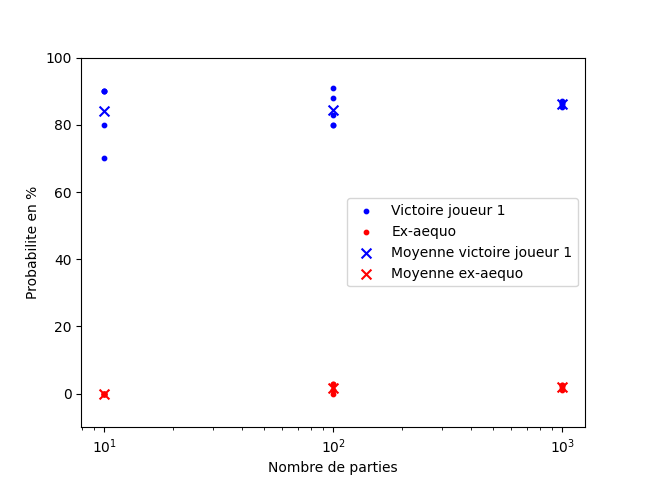
\includegraphics[width=0.75\textwidth]{ai_student_player=1_N=5.png}
\end{solutionbox}

\medskip

\emph{Cas 2:} Le joueur 1 joue \texttt{ai\_random.} et le joueur 2 joue \texttt{ai\_student.}

\begin{solutionbox}{100mm}
Insérez le graphe et mentionnez les probabilités moyennes obtenues pour $10^4$ parties.

\centering
La moyenne obtenue pour 5 repetitions de 10, 100 et 1000 parties lorsque l'IA joue en 2e position :
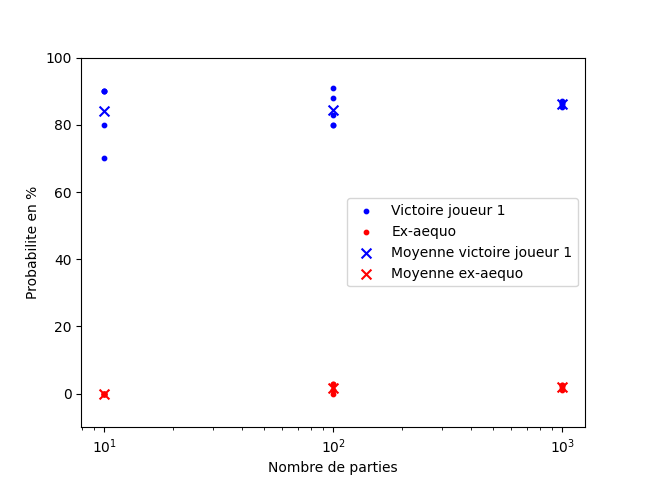
\includegraphics[width=0.75\textwidth]{ai_student_player=1_N=5.png}
\end{solutionbox}



\end{document}